% This LaTeX was auto-generated from MATLAB code.
% To make changes, update the MATLAB code and export to LaTeX again.

\documentclass{article}

\usepackage[utf8]{inputenc}
\usepackage[T1]{fontenc}
\usepackage{lmodern}
\usepackage{graphicx}
\usepackage{color}
\usepackage{hyperref}
\usepackage{amsmath}
\usepackage{amsfonts}
\usepackage{epstopdf}
\usepackage[table]{xcolor}
\usepackage{matlab}
\usepackage[paperheight=845pt,paperwidth=597pt,top=72pt,bottom=72pt,right=72pt,left=72pt,heightrounded]{geometry}

\sloppy
\epstopdfsetup{outdir=./}
\graphicspath{ {./HodgkinHuxley_media/} }

\matlabhastoc

\begin{document}

\label{TMP_9d7b}
\vspace{1em}

\label{TMP_706a}

\vspace{1em}
\matlabtableofcontents{目录}
\label{TMP_3105}
\vspace{1em}

\label{TMP_206a}
\vspace{1em}

\label{TMP_420b}
\matlabtitle{课题 1 : 可激发系统的模拟: Hodgkin-Huxley 神经元模型}


\vspace{1em}
\label{TMP_33cc}
\matlabheading{可激发系统}


\vspace{1em}

\vspace{1em}
\begin{par}
\begin{flushleft}
 可激发介质/系统 (excitable medium/system): 简言之就是具有 “可激励性”的介质, 也叫激励介质  
\end{flushleft}
\end{par}

\begin{par}
\begin{flushleft}
“可激励性”所对应的英文单词是“excitability”. 这个词在不同 的学科里有不同的译法: 物理学中叫可激发性, 医学中叫兴奋性、 敏感性, 生理学中叫刺激反应性 这里所指的“可激励性”是当介质 受到小扰动时, 介质很快恢复到平衡态 (静态); 但当扰动超过某一 阈值时, 介质将有一个快速又陡峭的响应, 呈现激发状态  
\end{flushleft}
\end{par}

\label{TMP_2538}
\matlabheading{神经元}

\begin{par}
\begin{flushleft}
大脑中神经元数目巨大 \textasciitilde{}10\textasciicircum{}11  
\end{flushleft}
\end{par}

\begin{par}
\begin{flushleft}
神经元形状及其多样  
\end{flushleft}
\end{par}


\vspace{1em}
\begin{par}
\begin{flushleft}
图中的标注及其翻译:
\end{flushleft}
\end{par}

\begin{par}
\begin{flushleft}
Soma :胞体
\end{flushleft}
\end{par}

\begin{par}
$$\textrm{Neurites}\textrm{:神经突}\left\lbrace \begin{array}{ll}
\textrm{Dendrites}\textrm{树突} & \\
\textrm{Axon}\textrm{:轴突} & 
\end{array}\right.$$
\end{par}

\label{TMP_60ae}
\matlabheading{神经元的可激发性}

\begin{par}
\begin{flushleft}
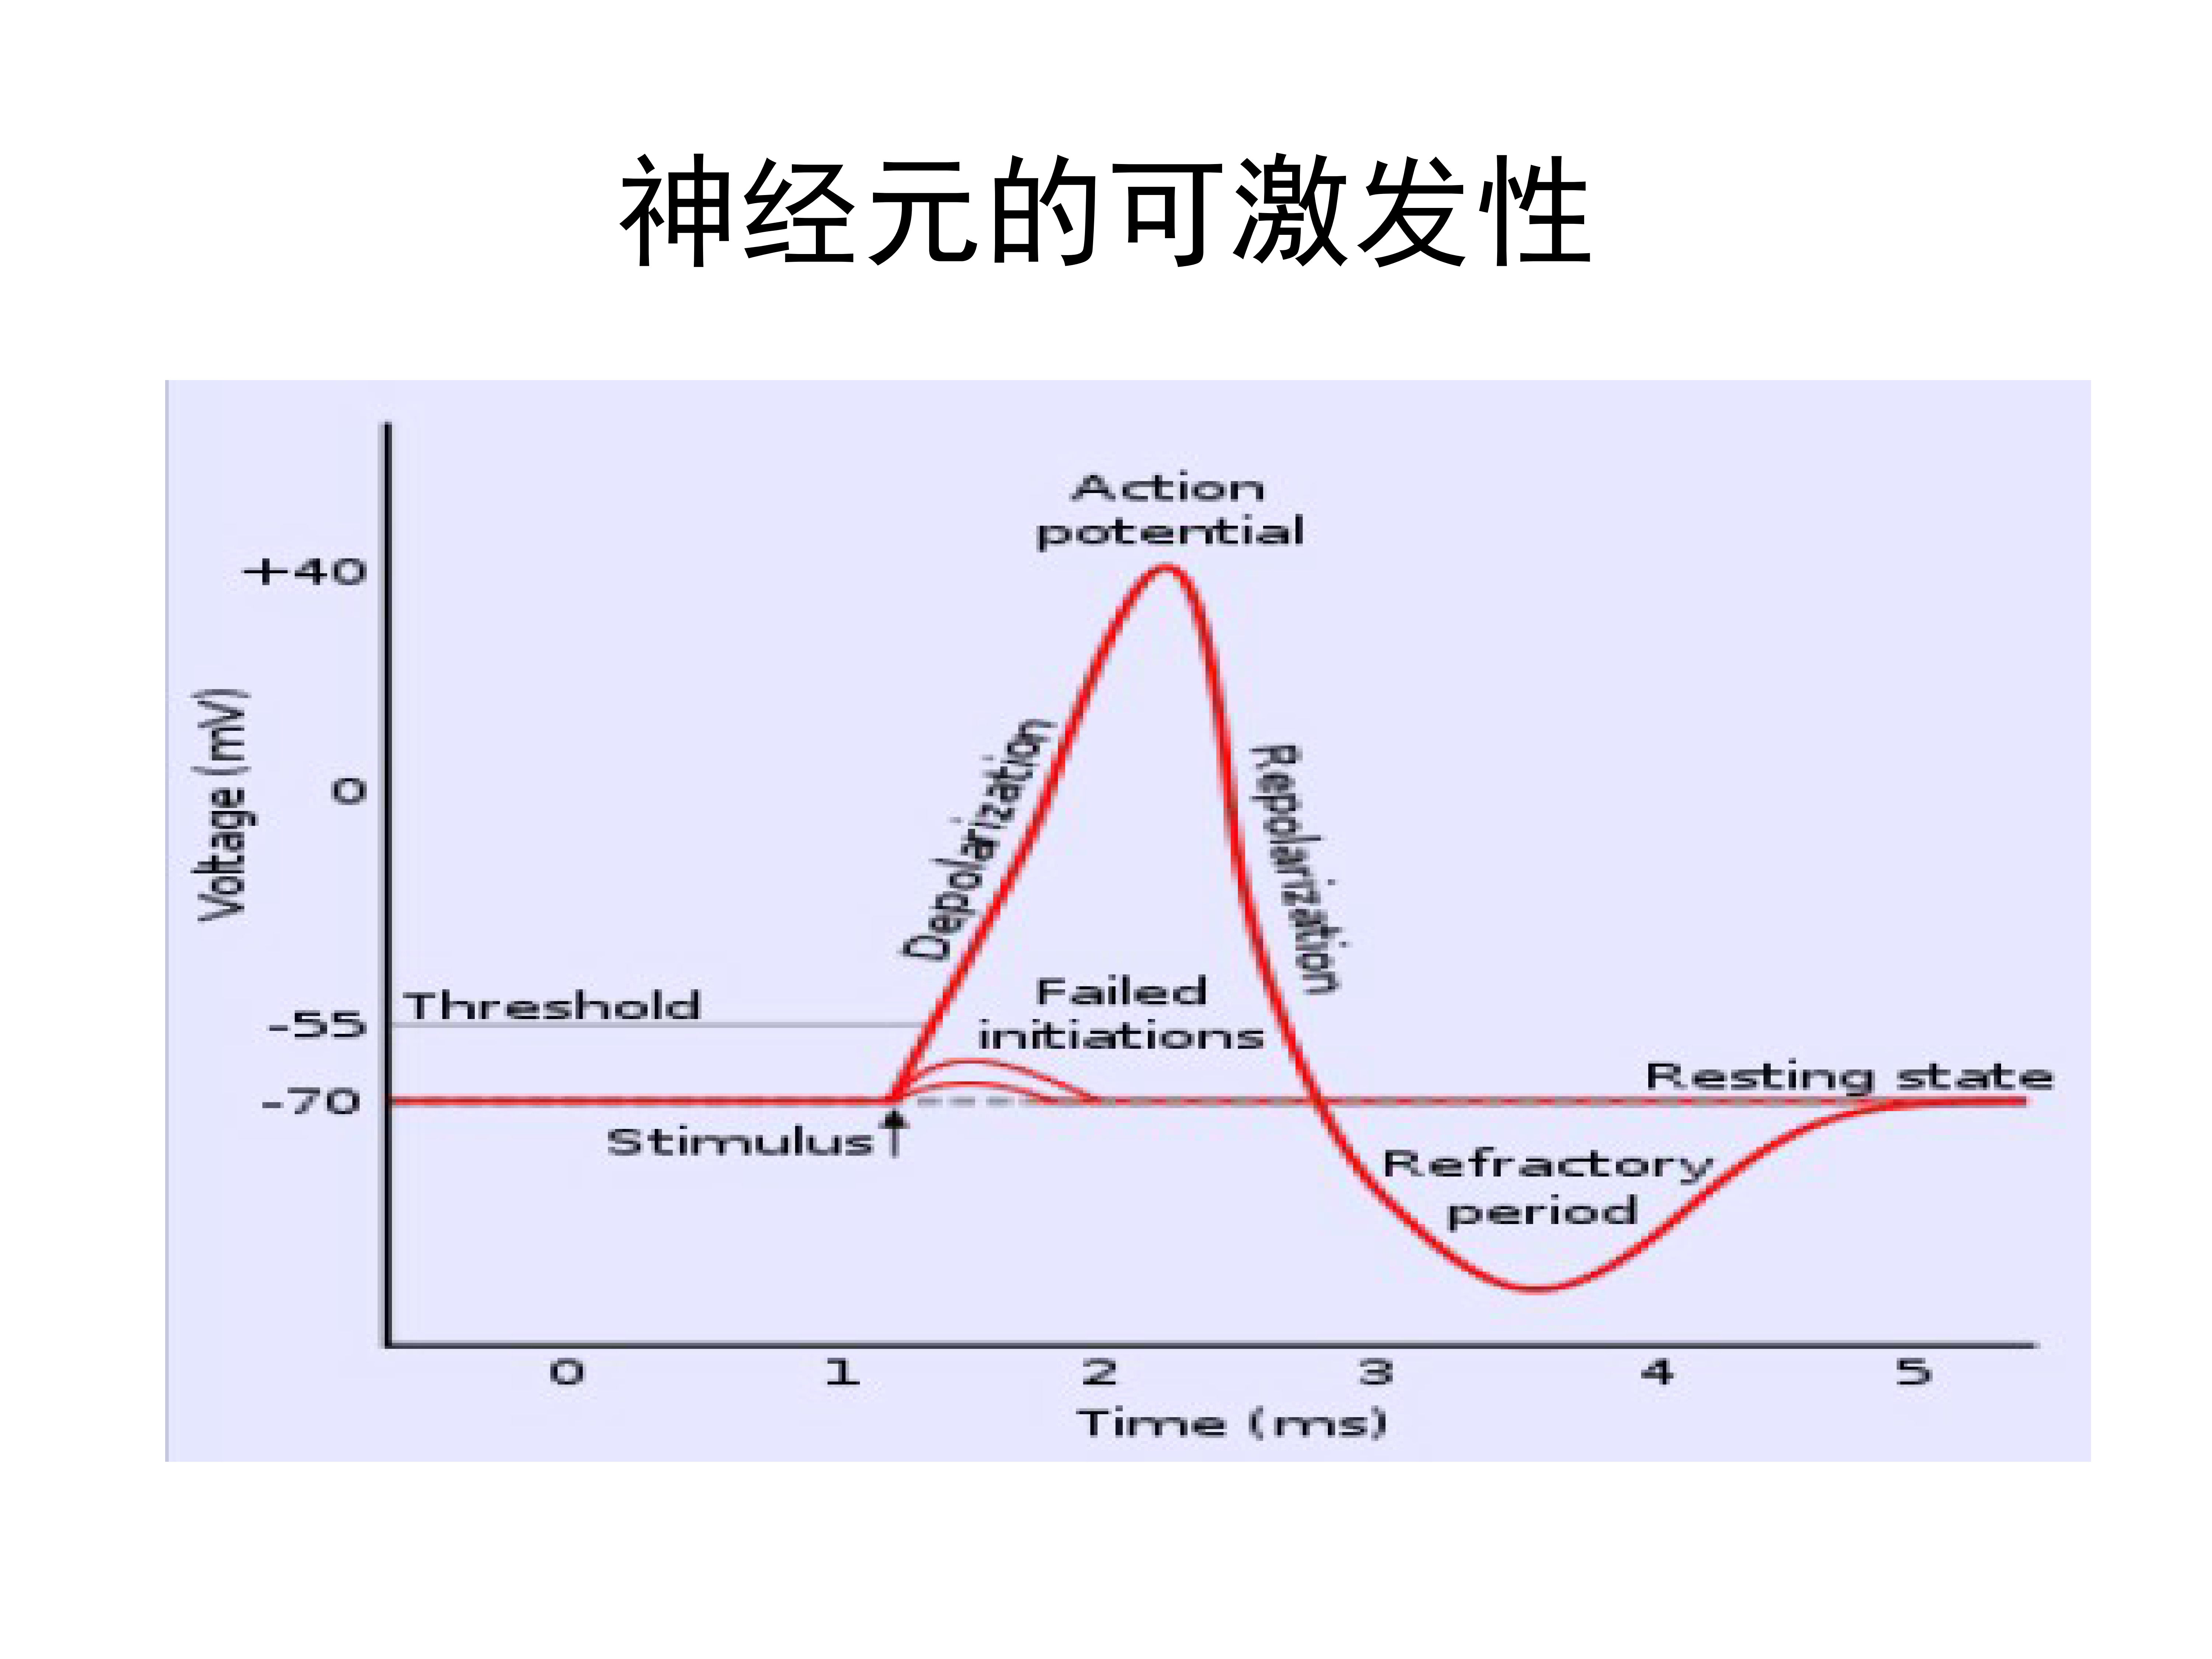
\includegraphics[width=\maxwidth{28.19869543401907em}]{image_0}
\end{flushleft}
\end{par}

\begin{par}
\begin{flushleft}
图中的标注及其翻译:
\end{flushleft}
\end{par}

\begin{par}
\begin{flushleft}
  Action potential :动作电势
\end{flushleft}
\end{par}

\begin{par}
\begin{flushleft}
  Depolarization :去极化
\end{flushleft}
\end{par}

\begin{par}
\begin{flushleft}
  Repolarization :复极化
\end{flushleft}
\end{par}

\begin{par}
\begin{flushleft}
  Failed initiations :失败的启动
\end{flushleft}
\end{par}

\begin{par}
\begin{flushleft}
  Threshold :阈值
\end{flushleft}
\end{par}

\begin{par}
\begin{flushleft}
  Resting state :静息态
\end{flushleft}
\end{par}

\begin{par}
\begin{flushleft}
  Stimulus :刺激
\end{flushleft}
\end{par}

\begin{par}
\begin{flushleft}
  Refractory period 不应期
\end{flushleft}
\end{par}


\vspace{1em}
\begin{par}
\begin{flushleft}
神经元在受到刺激时膜电位随时间变化的过程,称为\textbf{动作电势} 
\end{flushleft}
\end{par}


\vspace{1em}
\begin{par}
\begin{flushleft}
\textbf{Y轴 :} 电压,单位:mV 神经元细胞膜内外的电位差  
\end{flushleft}
\end{par}

\begin{par}
\begin{flushleft}
**X轴:**时间,单位:毫秒
\end{flushleft}
\end{par}

\begin{itemize}
\setlength{\itemsep}{-1ex}
   \item{\begin{flushleft} \textbf{三个电位水平 Potential Levels:} \end{flushleft}}
   \item{\begin{flushleft} \textbf{Resting state (静息态):} 约 -70 mV 神经元在未受刺激时的稳定电位 \end{flushleft}}
   \item{\begin{flushleft} \textbf{Threshold (阈值):} 约 -55 mV 临界电位 \end{flushleft}}
   \item{\begin{flushleft} \textbf{峰值:} 约 +40 mV 动作电势达到的最高电位 \end{flushleft}}
   \item{\begin{flushleft} \textbf{事件:} \end{flushleft}}
\end{itemize}

\begin{enumerate}
\setlength{\itemsep}{-1ex}
   \item{\begin{flushleft} \textbf{Stimulus (刺激):} 在 1 ms 稍过一点的位置,一个外部刺激被施加 \end{flushleft}}
   \item{\begin{flushleft} \textbf{Failed initiations (失败的启动):} 图中阈值下方的小波形  这表示刺激强度太弱,没有使膜电位达到 -55 mV 的阈值,因此无法触发一个完整的动作电势,电位很快就回落到静息态 \end{flushleft}}
   \item{\begin{flushleft} \textbf{Depolarization (去极化):} 当一个足够强的刺激使膜电位达到阈值 (-55 mV) 后,膜电位开始急剧上升,从负值变为正值,一直达到 +40 mV 的峰值 \end{flushleft}}
   \item{\begin{flushleft} \textbf{Action potential (动作电势):} 整个快速的电位“尖峰”(从去极化开始到复极化结束)被称为动作电势  图中的标签也特指其峰值 \end{flushleft}}
   \item{\begin{flushleft} \textbf{Repolarization (复极化):} 达到峰值后,膜电位迅速下降,从 +40 mV 降回负值 \end{flushleft}}
   \item{\begin{flushleft} \textbf{Refractory period (不应期):} 膜电位在复极化后,会短暂地降到比静息态(-70 mV)更低的水平  在这个时期,神经元对新的刺激反应能力降低(或完全不反应)  之后,电位会逐渐恢复到 -70 mV 的静息态   \end{flushleft}}
\end{enumerate}


\vspace{1em}

\vspace{1em}
\label{TMP_7d18}
\matlabheading{动作电势的特性}

\begin{par}
\begin{flushleft}
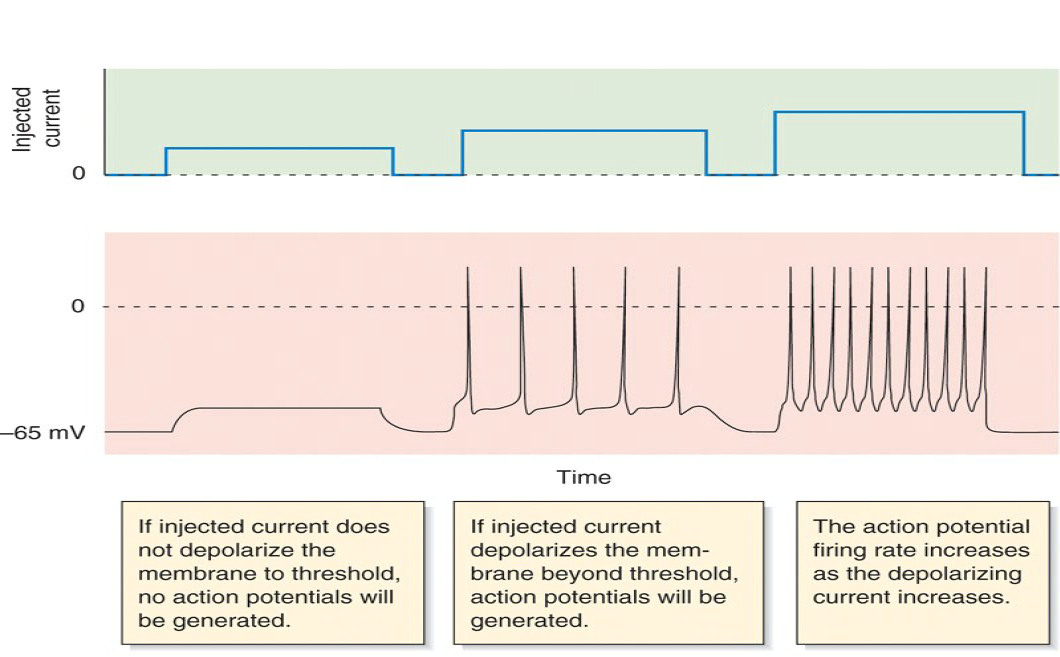
\includegraphics[width=\maxwidth{36.82890115403914em}]{image_1}
\end{flushleft}
\end{par}


\vspace{1em}
\begin{par}
\begin{flushleft}
  Injected current :注入电流
\end{flushleft}
\end{par}

\begin{par}
\begin{flushleft}
1.  If injected current does not depolarize the membrane to threshold, no action potentials will be generated.
\end{flushleft}
\end{par}

\begin{par}
\begin{flushleft}
    如果注入的电流没有使细胞膜去极化到阈值,则不会产生动作电势  
\end{flushleft}
\end{par}

\begin{par}
\begin{flushleft}
2.  If injected current depolarizes the membrane beyond threshold, action potentials will be generated.
\end{flushleft}
\end{par}

\begin{par}
\begin{flushleft}
    如果注入的电流使细胞膜去极化超过阈值,则会产生动作电势  
\end{flushleft}
\end{par}

\begin{par}
\begin{flushleft}
3.  The action potential firing rate increases as the depolarizing current increases.
\end{flushleft}
\end{par}

\begin{par}
\begin{flushleft}
    随着去极化电流的增加,动作电势的发放频率增加 
\end{flushleft}
\end{par}


\vspace{1em}
\label{TMP_66a1}
\matlabheading{神经元的数学建模}


\vspace{1em}
\label{TMP_8b9c}
\matlabheadingtwo{细胞膜与离子通道}


\vspace{1em}

\vspace{1em}

\vspace{1em}
\begin{par}
\begin{flushleft}
  channel 通道
\end{flushleft}
\end{par}

\begin{par}
\begin{flushleft}
  pore 孔隙
\end{flushleft}
\end{par}

\begin{par}
\begin{flushleft}
  lipid bilayer 脂双层
\end{flushleft}
\end{par}


\vspace{1em}
\label{TMP_15af}
\matlabheadingtwo{等效电路}

\begin{par}
\begin{flushleft}
等效成了三个电阻和一个电容并联,并且在每个电阻的回路串上电池,每个电迟代表了对应离子的能斯特电位,电阻则代表了离子泵的耗能
\end{flushleft}
\end{par}

\begin{par}
\begin{flushleft}
这个模型中的能量来源是电池提供的,即营养物质的摄入
\end{flushleft}
\end{par}

\label{TMP_5824}
\matlabheadingthree{PPT上指出的公式}

\begin{par}
\begin{flushleft}
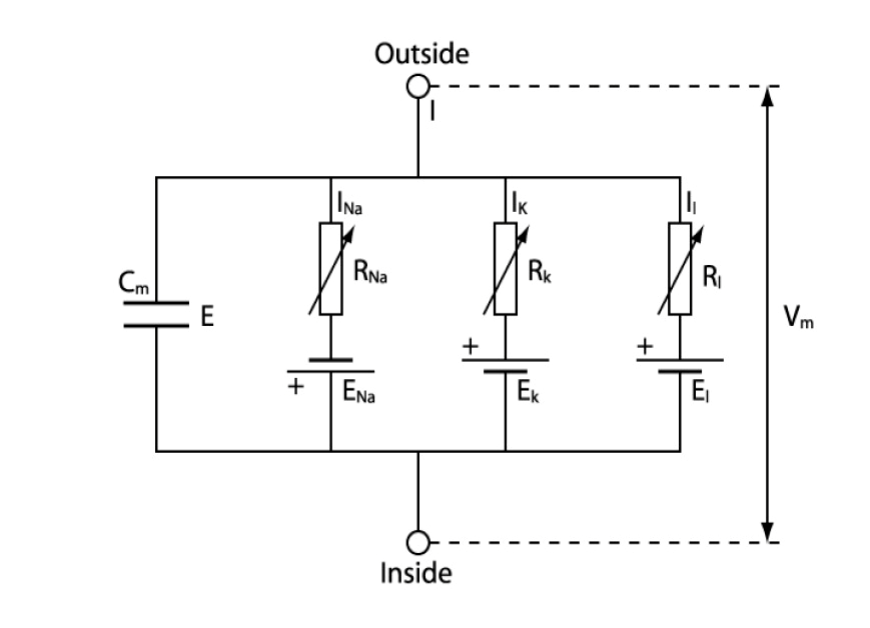
\includegraphics[width=\maxwidth{22.880080280983442em}]{image_2}
\end{flushleft}
\end{par}

\begin{par}
$$C_m \frac{dV_m }{dt}+I_{ion} =I_{ext}$$
\end{par}

\begin{par}
$$I_{ion} =\sum_k I_k =\sum_k G_k (V_m -E_k )\ldotp$$
\end{par}

\begin{par}
\begin{flushleft}
这里的$I_{ext}$ 是外部总电流,$I_{ion}$指离子电流之和
\end{flushleft}
\end{par}

\begin{par}
\begin{flushleft}
离子有三种,Na, K,还有泄露(主要是氯离子)
\end{flushleft}
\end{par}

\begin{par}
\begin{flushleft}
 $V_m$ 是指内外模的电势差,$G_k$指电导
\end{flushleft}
\end{par}

\label{TMP_8f16}
\matlabheadingthree{PPT中给出的微分方程是}

\begin{par}
$$\left\lbrace \begin{array}{l}
C_m \frac{dV}{dt}=-g_L (V-E_L )-{\bar{g} }_{Na} m^3 h(V-E_{Na} )-{\bar{g} }_K n^4 (V-E_K )+I_{app} \\
\frac{dm}{dt}=\alpha_m (V)(1-m)-\beta_m (V)m\\
\frac{dh}{dt}=\alpha_h (V)(1-h)-\beta_h (V)h\\
\frac{dn}{dt}=\alpha_n (V)(1-n)-\beta_n (V)n
\end{array}\right.$$
\end{par}


\vspace{1em}
\begin{par}
\begin{flushleft}
HH 模型描述了动作电势的发生过程  
\end{flushleft}
\end{par}

\label{TMP_4826}
\matlabheadingthree{PPT中给出的参数是}

\begin{par}
\begin{flushleft}
电容:$C=1\mu {\textrm{F/cm}}^2$
\end{flushleft}
\end{par}


\vspace{1em}
\begin{par}
\begin{flushleft}
各离子的能斯特电位和对应的电导:
\end{flushleft}
\end{par}

\begin{par}
$$\begin{array}{lrr}
\hline
x & E_x \;\textrm{[mV]} & g_x {\;\textrm{[mS}\;\textrm{/}\;\textrm{cm}}^2 \textrm{]}\\
\hline
\textrm{Na} & 55 & 40\\
\textrm{K} & -77 & 35\\
\textrm{L} & -65 & 0.3\\
\hline
\end{array}$$
\end{par}

\begin{par}
\begin{flushleft}
对应的 alpha和beta函数:
\end{flushleft}
\end{par}

\begin{par}
$$\begin{array}{lcc}
\hline
x & \alpha_x (u/\;\textrm{mV}){\;\textrm{[ms}}^{-1} \textrm{]} & \beta_x (u/\cdot \;\textrm{mV}){\;\textrm{[ms}}^{-1} \textrm{]}\\
\hline
n & 0.02(u-25)/[1-e^{-(u-25)/9} ] & -0.002(u-25)/[1-e^{(u-25)/9} ]\\
m & 0.182(u+35)/[1-e^{-(u+35)/9} ] & -0.124(u+35)/[1-e^{(u+35)/9} ]\\
h & 0.25e^{-(u+90)/12}  & 0.25e^{(u+62)/6} /e^{(u+90)/12} \\
\hline
\end{array}$$
\end{par}


\vspace{1em}
\label{TMP_5d84}
\matlabheadingthree{文献中给出的微分方程:}


\vspace{1em}
\begin{par}
\begin{flushleft}
根据《Energy and information in Hodgkin-Huxley neurons》A. Moujahid, A. d’Anjou, and F. J. Torrealdea
\end{flushleft}
\end{par}

\begin{par}
\begin{flushleft}
突奇-赫胥黎HH模型描述了无动作电位传播的鱿鱼巨轴突,将其视为通用神经元动力学的代表,遵循以下微分方程:
\end{flushleft}
\end{par}

\begin{par}
$$\begin{array}{rcl}
C\dot{V}  & = & -i_{Na} -i_K -i_l +I,\\
\dot{m}  & = & \alpha_m (V)(1-m)-\beta_m (V)m,\\
\dot{n}  & = & \alpha_n (V)(1-n)-\beta_n (V)n,\\
\dot{h}  & = & \alpha_h (V)(1-h)-\beta_h (V)h,
\end{array}~~(1)$$
\end{par}


\vspace{1em}
\begin{par}
\begin{flushleft}
其中 $V$ 是以 $mV$ 为单位的\textbf{膜电位},$C$ 是以 $\mu F$ 为单位的\textbf{膜电容}
\end{flushleft}
\end{par}

\begin{par}
\begin{flushleft}
$I$ 是以 $\mu A/cm^2$ 为单位的\textbf{总膜电流密度}
\end{flushleft}
\end{par}

\begin{par}
\begin{flushleft}
而 $m$、$n$ 和 $h\,$ 是无量纲变量
\end{flushleft}
\end{par}

\begin{par}
\begin{flushleft}
分别表示\textbf{膜内侧钠激活分子的比例}、\textbf{膜内侧钾激活粒子的比例}
\end{flushleft}
\end{par}

\begin{par}
\begin{flushleft}
以及\textbf{膜外侧钠失活分子的比例} 。
\end{flushleft}
\end{par}


\vspace{1em}
\begin{par}
\begin{flushleft}
A. Moujahid文章中的钠、钾和泄漏 (主要是氯) 的离子电流,分别记为 $i_{Na}$、$i_K$
\end{flushleft}
\end{par}

\begin{par}
\begin{flushleft}
和 $i_l$,由下式给出:
\end{flushleft}
\end{par}


\vspace{1em}
\begin{par}
$$\begin{array}{rcl}
i_{Na}  & = & g_{Na} m^3 h(V-E_{Na} ),\\
i_K  & = & g_K n^4 (V-E_K ),\\
i_l  & = & g_l (V-E_l ),
\end{array}~~(2)$$
\end{par}


\vspace{1em}
\begin{par}
\begin{flushleft}
其中 $g_{Na}$、$g_K$ 和 $g_l$ 是各自离子通道电导的最大可能值,并且
\end{flushleft}
\end{par}

\begin{par}
\begin{flushleft}
$E_{Na}$、$E_K$ 和 $E_l$ 离子在神经元静态状态下的能斯特电位。在这
\end{flushleft}
\end{par}

\begin{par}
\begin{flushleft}
项工作中,我们给出了这些参数的标准常数值,这些值在下表中给出。
\end{flushleft}
\end{par}

\label{TMP_5a34}
\matlabheadingthree{文献中给出的参数是}

\begin{par}
\begin{flushleft}
膜电容为  $C=1\mu {\textrm{F/cm}}^2$
\end{flushleft}
\end{par}

\begin{par}
\begin{flushleft}
电压标度被偏移,使得静息电位为零
\end{flushleft}
\end{par}

\begin{par}
$$\begin{array}{lrr}
\hline
x & g_x {\;\textrm{(mS/cm}}^2 \textrm{)} & E_x \;\textrm{(mV)}\\
\hline
\textrm{Na} & 120 & 115\\
\textrm{K} & 36 & -12\\
\textrm{l} & 0.3 & 10.6\\
\hline
\end{array}$$
\end{par}

\begin{par}
\begin{flushleft}
A. Moujahid文章中随时间变化的变量alpha和beta函数是
\end{flushleft}
\end{par}


\vspace{1em}
\begin{par}
$$\begin{array}{rcl}
\alpha_m (V) & = & (2.5-0.1V)/[\exp (2.5-0.1V)-1],\\
\beta_m (V) & = & 4\exp (-V/18),\\
\alpha_n (V) & = & (0.1-0.01V)/[\exp (1-0.1V)-1],\\
\beta_n (V) & = & 0.125\exp (-V/80),\\
\alpha_h (V) & = & 0.07\exp (-V/20),\\
\beta_h (V) & = & 1/[\exp (3-0.1V)+1].
\end{array}$$
\end{par}


\vspace{1em}

\label{TMP_9717}
\matlabheading{任务 1:研究不同刺激强度下神经元膜电势的变化}


\vspace{1em}

\vspace{1em}
\begin{par}
\begin{flushleft}
  请利用四阶 Rung=Kutta 算法求解 HH 方程, 并研究不同刺激强度下神经元膜电势的变化, 借此理解可激发系统的响应特性  
\end{flushleft}
\end{par}


\vspace{1em}
\begin{par}
\begin{flushleft}
脉冲刺激 或 直流刺激
\end{flushleft}
\end{par}


\vspace{1em}
\begin{par}
\begin{flushleft}
解答:
\end{flushleft}
\end{par}

\begin{par}
\begin{flushleft}
我们将分别对 脉冲刺激 或 直流刺激 使用PPT中的参数和方程 文献中对应的参数和方程 ,因此组合后结果应该有四种:
\end{flushleft}
\end{par}

\begin{par}
\begin{flushleft}
我们先复现PPT中的结果:
\end{flushleft}
\end{par}

\label{TMP_4e59}
\vspace{1em}


\vspace{1em}


\vspace{1em}
\label{TMP_857b}
\matlabheadingtwo{脉冲刺激1-使用PPT中的参数和方程}

\begin{par}
\begin{flushleft}
此时的常数为
\end{flushleft}
\end{par}

\label{TMP_6c4e}
\begin{par}
\begin{flushleft}
PPT中给出的参数是
\end{flushleft}
\end{par}

\begin{par}
\begin{flushleft}
电容:$C=1\mu {\textrm{F/cm}}^2$
\end{flushleft}
\end{par}

\begin{matlabcode}
clc;clear;
C=1;
\end{matlabcode}

\begin{par}
\begin{flushleft}
各离子的能斯特电位和对应的电导:
\end{flushleft}
\end{par}

\begin{par}
$$\begin{array}{lrr}
\hline
x & E_x \;\textrm{[mV]} & g_x {\;\textrm{[mS}\;\textrm{/}\;\textrm{cm}}^2 \textrm{]}\\
\hline
\textrm{Na} & 55 & 40\\
\textrm{K} & -77 & 35\\
\textrm{L} & -65 & 0.3\\
\hline
\end{array}$$
\end{par}

\begin{matlabcode}
E.Na=55;E.K=-77;E.L=-65;
g.Na=40;g.K=35;g.L=0.3;

% E.Na=115;E.K=-12;E.L=10.6;
% g.Na=120;g.K=36;g.L=0.3;
\end{matlabcode}

\begin{par}
\begin{flushleft}
对应的 alpha和beta函数:
\end{flushleft}
\end{par}

\begin{par}
$$\begin{array}{lcc}
\hline
x & \alpha_x (u/\;\textrm{mV}){\;\textrm{[ms}}^{-1} \textrm{]} & \beta_x (u/\cdot \;\textrm{mV}){\;\textrm{[ms}}^{-1} \textrm{]}\\
\hline
n & 0.02(u-25)/[1-e^{-(u-25)/9} ] & -0.002(u-25)/[1-e^{(u-25)/9} ]\\
m & 0.182(u+35)/[1-e^{-(u+35)/9} ] & -0.124(u+35)/[1-e^{(u+35)/9} ]\\
h & 0.25e^{-(u+90)/12}  & 0.25e^{(u+62)/6} /e^{(u+90)/12} \\
\hline
\end{array}$$
\end{par}

\begin{matlabcode}
Alpha.n=@(u) 0.02*(u-25)/(1-exp(-(u-25)/9));
Alpha.m=@(u) 0.182*(u+35)/(1-exp(-(u+35)/9));
Alpha.h=@(u) 0.25*exp(-(u+90)/12);
Beta.n=@(u) -0.002*(u-25)/(1-exp((u-25)/9));
Beta.m=@(u) -0.124*(u+35)/(1-exp((u+35)/9));
Beta.h=@(u) 0.25*exp((u+62)/6)/exp((u+90)/12);

% Alpha.n=@(u) (0.1 - 0.01.*u) ./ (exp(1 - 0.1.*u) - 1);
% Alpha.m=@(u) (2.5 - 0.1.*u) ./ (exp(2.5 - 0.1.*u) - 1);
% Alpha.h=@(u) 0.07 .* exp(-u./20);
% Beta.n=@(u) 0.125 .* exp(-u./80);
% Beta.m=@(u) 4 .* exp(-u./18);
% Beta.h=@(u) 1 ./ (exp(3 - 0.1.*u) + 1);

fs= 4000;%采样频率
T=200;%总时长(ms)
A=15;%刺激电流强度

% I_ext = @(u) 0+(20<=u & u<= 30).*A...
%     +(40<=u & u<= 50).*A/2 ...
%     +(60<=u & u<= 70).*A/4 ...
%     +(80<=u & u<= 90).*A/8 ...
%     +(100<=u & u<= 110).*A/10 ...
%     +(120<=u & u<= 130).*A/12 ...
%     +(140<=u & u<= 150).*A/14 ...
%     +(160<=u & u<= 170).*A/16 ...
%     +(180<=u & u<= 190).*A/20 ...
% ;%脉冲刺激向量
Center=(25:20:185)';%脉冲中心位置,取转置是因为要列向量
Scale=[1,1/2,1/4,1/8,1/10,1/12,1/14,1/16,1/20]';%脉冲高度
Amplitude=A*Scale;
D1=[Center,Amplitude];%用给pulstran函数,第一列脉冲中心,第二列脉冲高度
PulWidth=10;%脉冲刺激宽度为10ms
PulShap=@(t) rectpuls(t,PulWidth);%脉冲刺激函数
I_ext=@(u) pulstran(u,D1,PulShap);

Task1I2V(C,E,g,Alpha,Beta, ...
    'fs',fs, ...
    'T',T, ...
    'A',A, ...
    'I_ext',I_ext);
\end{matlabcode}
\begin{matlaboutput}
此时使用的参数为:
 C: 1.0000 
g的结构体:
    Na: 40
     K: 35
     L: 0.300000000000000

E的结构体:
    Na: 55
     K: -77
     L: -65

Alpha函数的结构体:
    n: @(u)0.02*(u-25)/(1-exp(-(u-25)/9))
    m: @(u)0.182*(u+35)/(1-exp(-(u+35)/9))
    h: @(u)0.25*exp(-(u+90)/12)

Beta函数的结构体:
    n: @(u)-0.002*(u-25)/(1-exp((u-25)/9))
    m: @(u)-0.124*(u+35)/(1-exp((u+35)/9))
    h: @(u)0.25*exp((u+62)/6)/exp((u+90)/12)

外部刺激电流:
    @(u)pulstran(u,D1,PulShap)


下图是外部电流刺激的时域图
\end{matlaboutput}
\begin{center}
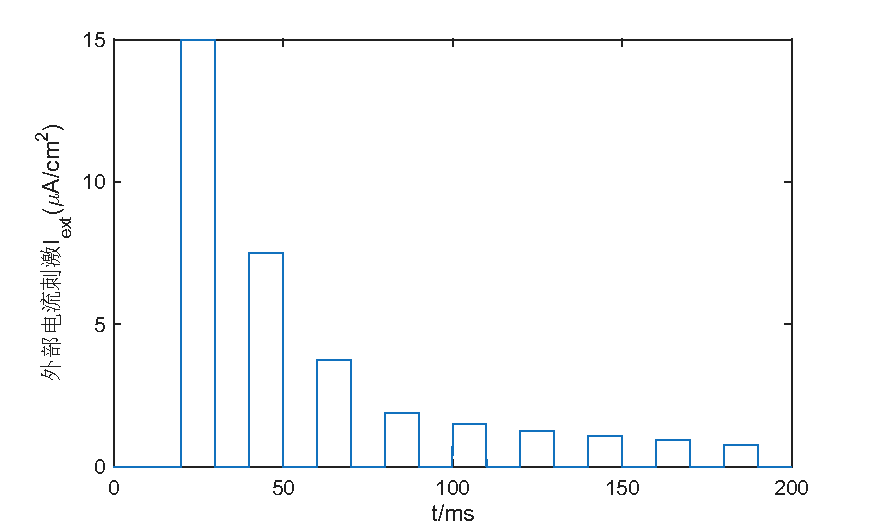
\includegraphics[width=\maxwidth{56.196688409433015em}]{figure_0.pdf}
\end{center}
\begin{matlaboutput}
下图是膜电压与时间的关系: 
\end{matlaboutput}
\begin{center}
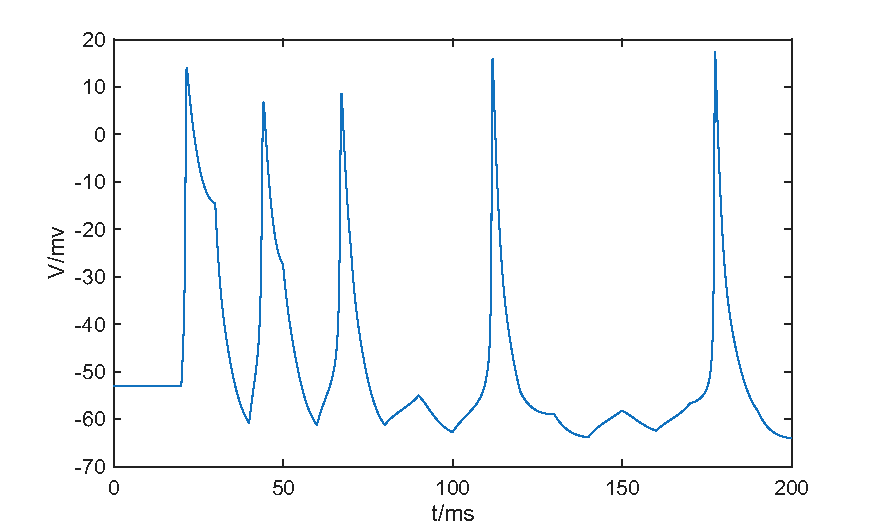
\includegraphics[width=\maxwidth{56.196688409433015em}]{figure_1.pdf}
\end{center}


\label{TMP_26d4}
\matlabheadingtwo{脉冲刺激2-使用PPT中的参数和方程}

\begin{matlabcode}
% I_ext = @(u) 0+(20<=u & u<= 30).*A...
%     +(40<=u & u<= 50).*A/2 ...
%     +(60<=u & u<= 70).*A/4 ...
%     +(80<=u & u<= 90).*A/8 ...
%     +(100<=u & u<= 110).*A/16 ...
%     +(120<=u & u<= 130).*A/32 ...
A=5;
%脉冲刺激向量
Center=(25:20:185)';%脉冲中心位置,取转置是因为要列向量
% Scale=0.7.^(0:1:8)';%脉冲高度;
Scale=linspace(1,0,9)';
Amplitude=A*Scale;
D1=[Center,Amplitude];%用给pulstran函数,第一列脉冲中心,第二列脉冲高度
PulWidth=10;%脉冲刺激宽度为10ms
PulShap=@(t) rectpuls(t,PulWidth);%脉冲刺激函数
I_ext=@(u) pulstran(u,D1,PulShap);

%脉冲刺激向量

Task1I2V(C,E,g,Alpha,Beta, ...
    'fs',fs, ...
    'T',T, ...
    'A',A, ...
    'I_ext',I_ext);
\end{matlabcode}
\begin{matlaboutput}
此时使用的参数为:
 C: 1.0000 
g的结构体:
    Na: 40
     K: 35
     L: 0.300000000000000

E的结构体:
    Na: 55
     K: -77
     L: -65

Alpha函数的结构体:
    n: @(u)0.02*(u-25)/(1-exp(-(u-25)/9))
    m: @(u)0.182*(u+35)/(1-exp(-(u+35)/9))
    h: @(u)0.25*exp(-(u+90)/12)

Beta函数的结构体:
    n: @(u)-0.002*(u-25)/(1-exp((u-25)/9))
    m: @(u)-0.124*(u+35)/(1-exp((u+35)/9))
    h: @(u)0.25*exp((u+62)/6)/exp((u+90)/12)

外部刺激电流:
    @(u)pulstran(u,D1,PulShap)


下图是外部电流刺激的时域图
\end{matlaboutput}
\begin{center}
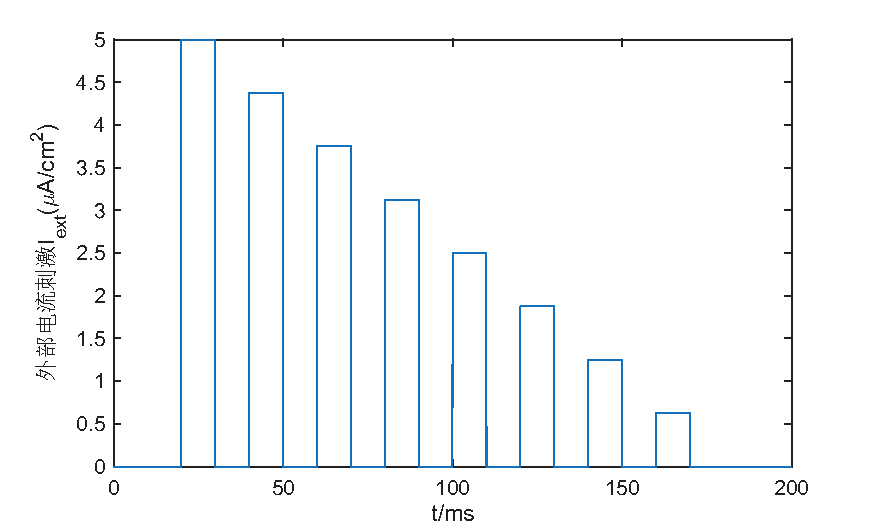
\includegraphics[width=\maxwidth{56.196688409433015em}]{figure_2.pdf}
\end{center}
\begin{matlaboutput}
下图是膜电压与时间的关系: 
\end{matlaboutput}
\begin{center}
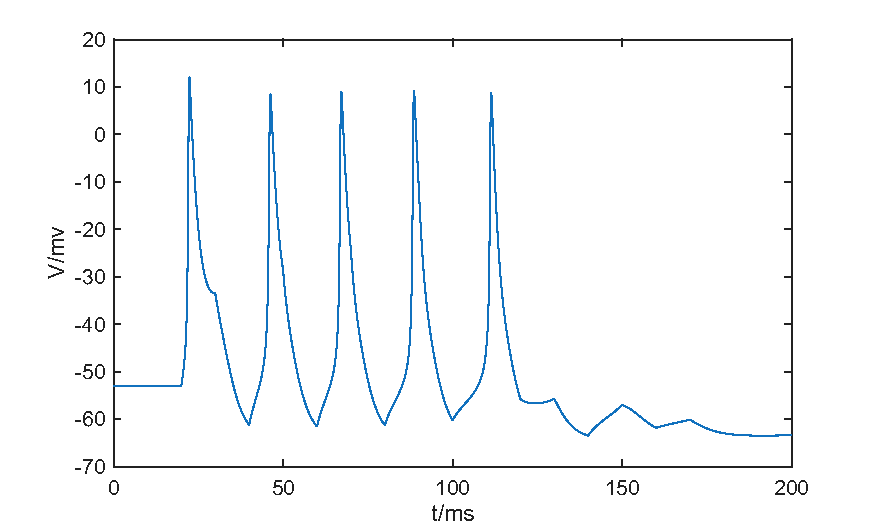
\includegraphics[width=\maxwidth{56.196688409433015em}]{figure_3.pdf}
\end{center}


\vspace{1em}
\begin{par}
\begin{flushleft}
由此可发现,在刺激电流大于某一阈值时,无论刺激电流大小都会得到相同的膜电压动作电位变化
\end{flushleft}
\end{par}

\begin{par}
\begin{flushleft}
而我们通过一个等比数列递减的外部电流刺激近似得出,大概在第七次时就不能得到膜电压了
\end{flushleft}
\end{par}

\begin{par}
\begin{flushleft}
此时的电流大小为大概在 2.5\textasciitilde{}1.875 mu A/cm\textasciicircum{}2 之间
\end{flushleft}
\end{par}

\begin{matlabcode}
Amplitude(5:6)
\end{matlabcode}
\begin{matlaboutput}
ans = 2x1
   2.500000000000000
   1.875000000000000

\end{matlaboutput}


\vspace{1em}

\label{TMP_085d}
\vspace{1em}

\label{TMP_743b}
\matlabheadingtwo{直流刺激-使用PPT中的参数和方程}

\begin{matlabcode}
% A=5;
% %脉冲刺激向量
% Center=(25:20:185)';%脉冲中心位置,取转置是因为要列向量
% % Scale=0.7.^(0:1:8)';%脉冲高度;
% Scale=linspace(1,0,9)';
% Amplitude=A*Scale;
% D1=[Center,Amplitude];%用给pulstran函数,第一列脉冲中心,第二列脉冲高度
% PulWidth=10;%脉冲刺激宽度为10ms
% PulShap=@(t) rectpuls(t,PulWidth);%脉冲刺激函数
% I_ext=@(u) pulstran(u,D1,PulShap);
A=10;
I_ext = @(u) 0+(20<=u & u<= 150).*A;

%脉冲刺激向量

Task1I2V(C,E,g,Alpha,Beta, ...
    'fs',fs, ...
    'T',T, ...
    'A',A, ...
    'I_ext',I_ext);
\end{matlabcode}
\begin{matlaboutput}
此时使用的参数为:
 C: 1.0000 
g的结构体:
    Na: 40
     K: 35
     L: 0.300000000000000

E的结构体:
    Na: 55
     K: -77
     L: -65

Alpha函数的结构体:
    n: @(u)0.02*(u-25)/(1-exp(-(u-25)/9))
    m: @(u)0.182*(u+35)/(1-exp(-(u+35)/9))
    h: @(u)0.25*exp(-(u+90)/12)

Beta函数的结构体:
    n: @(u)-0.002*(u-25)/(1-exp((u-25)/9))
    m: @(u)-0.124*(u+35)/(1-exp((u+35)/9))
    h: @(u)0.25*exp((u+62)/6)/exp((u+90)/12)

外部刺激电流:
    @(u)0+(20<=u&u<=150).*A


下图是外部电流刺激的时域图
\end{matlaboutput}
\begin{center}
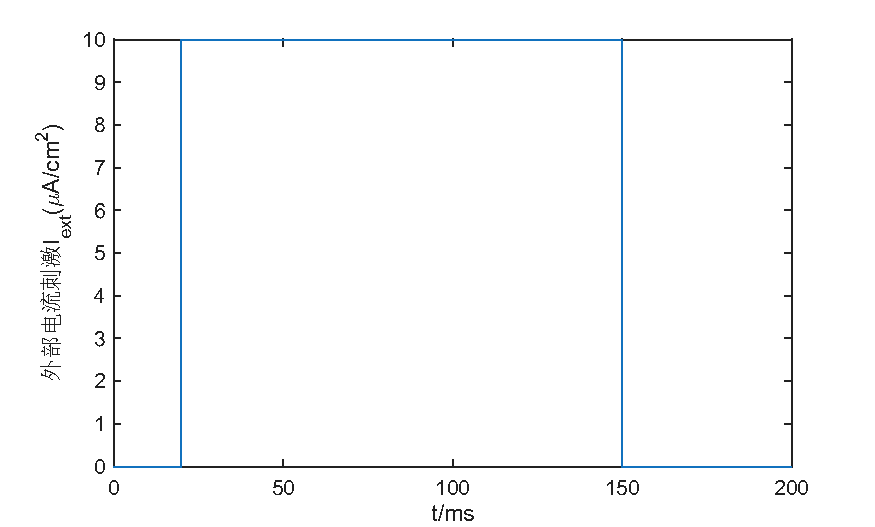
\includegraphics[width=\maxwidth{56.196688409433015em}]{figure_4.pdf}
\end{center}
\begin{matlaboutput}
下图是膜电压与时间的关系: 
\end{matlaboutput}
\begin{center}
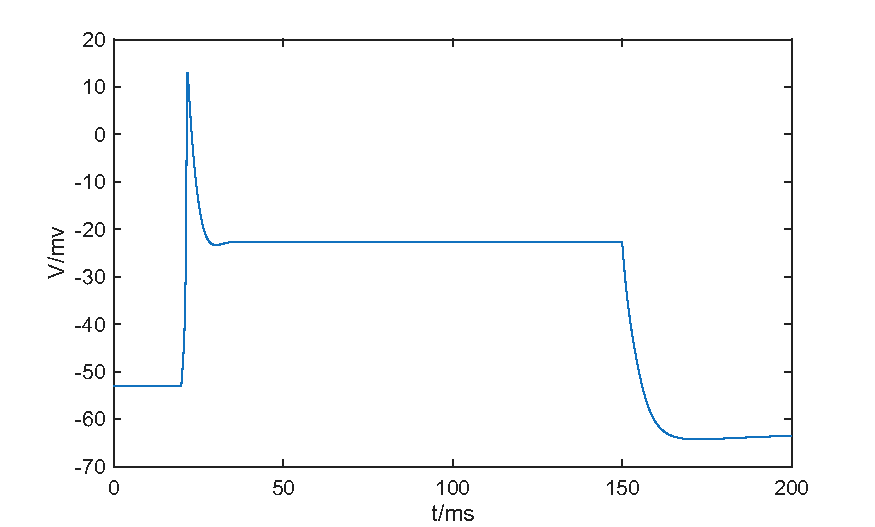
\includegraphics[width=\maxwidth{56.196688409433015em}]{figure_5.pdf}
\end{center}

\begin{par}
\begin{flushleft}
我们发现使用PPT中的参数和alpha,beta函数无法在直流时产生多个动作电位
\end{flushleft}
\end{par}

\begin{par}
\begin{flushleft}
这是因为PPT中所使用的模型参数有问题导致的,我们在下面使用另一组参数,只改动常数和alpha beta函数
\end{flushleft}
\end{par}

\begin{par}
\begin{flushleft}
可以立刻得到直流时的多个动作电位
\end{flushleft}
\end{par}


\label{TMP_566d}
\vspace{1em}

\label{TMP_34d4}
\matlabheadingtwo{脉冲刺激-使用文献中的参数和方程}


\vspace{1em}
\begin{par}
\begin{flushleft}
《Energy and information in Hodgkin-Huxley neurons》A. Moujahid, A. d’Anjou, and F. J. Torrealdea
\end{flushleft}
\end{par}

\label{TMP_6c4e}
\begin{par}
\begin{flushleft}
中给出的参数是
\end{flushleft}
\end{par}

\begin{par}
\begin{flushleft}
电容:$C=1\mu {\textrm{F/cm}}^2$
\end{flushleft}
\end{par}

\begin{matlabcode}
clc;clear
C=1;
\end{matlabcode}

\begin{par}
\begin{flushleft}
各离子的能斯特电位和对应的电导:
\end{flushleft}
\end{par}

\begin{par}
$$\begin{array}{lrr}
\hline
x & E_x \;\textrm{[mV]} & g_x {\;\textrm{[mS}\;\textrm{/}\;\textrm{cm}}^2 \textrm{]}\\
\hline
\textrm{Na} & 115 & 120\\
\textrm{K} & -12 & 36\\
\textrm{L} & 10.6 & 0.3\\
\hline
\end{array}$$
\end{par}

\begin{matlabcode}
% E.Na=55;E.K=-77;E.L=-65;
% g.Na=40;g.K=35;g.L=0.3;

E.Na=115;E.K=-12;E.L=10.6;
g.Na=120;g.K=36;g.L=0.3;
\end{matlabcode}

\begin{par}
\begin{flushleft}
对应的 alpha和beta函数:
\end{flushleft}
\end{par}

\begin{par}
$$\begin{array}{lcc}
\hline
x & \alpha_x (u/\;\textrm{mV}){\;\textrm{[ms}}^{-1} \textrm{]} & \beta_x (u/\cdot \;\textrm{mV}){\;\textrm{[ms}}^{-1} \textrm{]}\\
\hline
n & (0.1-0.01u)/[\exp (1-0.1u)-1] & 0.125\exp (-u/80)\\
m & (2.5-0.1u)/[\exp (2.5-0.1u)-1] & 4\exp (-u/18)\\
h & 0.07\exp (-u/20) & 1/[\exp (3-0.1u)+1]\\
\hline
\end{array}$$
\end{par}

\begin{matlabcode}
% Alpha.n=@(u) 0.02*(u-25)/(1-exp(-(u-25)/9));
% Alpha.m=@(u) 0.182*(u+35)/(1-exp(-(u+35)/9));
% Alpha.h=@(u) 0.25*exp(-(u+90)/12);
% Beta.n=@(u) -0.002*(u-25)/(1-exp((u-25)/9));
% Beta.m=@(u) -0.124*(u+35)/(1-exp((u+35)/9));
% Beta.h=@(u) 0.25*exp((u+62)/6)/exp((u+90)/12);

Alpha.n=@(u) (0.1 - 0.01.*u) ./ (exp(1 - 0.1.*u) - 1);
Alpha.m=@(u) (2.5 - 0.1.*u) ./ (exp(2.5 - 0.1.*u) - 1);
Alpha.h=@(u) 0.07 .* exp(-u./20);
Beta.n=@(u) 0.125 .* exp(-u./80);
Beta.m=@(u) 4 .* exp(-u./18);
Beta.h=@(u) 1 ./ (exp(3 - 0.1.*u) + 1);
A=5;
%脉冲刺激向量
Center=(25:20:185)';%脉冲中心位置,取转置是因为要列向量
% Scale=0.7.^(0:1:8)';%脉冲高度;
Scale=linspace(1,0,9)';
Amplitude=A*Scale;
D1=[Center,Amplitude];%用给pulstran函数,第一列脉冲中心,第二列脉冲高度
PulWidth=10;%脉冲刺激宽度为10ms
PulShap=@(t) rectpuls(t,PulWidth);%脉冲刺激函数
I_ext=@(u) pulstran(u,D1,PulShap);
%脉冲刺激向量

fs= 4000;%采样频率
T=200;%总时长(ms)
A=15;%刺激电流强度

Task1I2V(C,E,g,Alpha,Beta, ...
    'fs',fs, ...
    'T',T, ...
    'A',A, ...
    'I_ext',I_ext);
\end{matlabcode}
\begin{matlaboutput}
此时使用的参数为:
 C: 1.0000 
g的结构体:
    Na: 120
     K: 36
     L: 0.300000000000000

E的结构体:
    Na: 115
     K: -12
     L: 10.600000000000000

Alpha函数的结构体:
    n: @(u)(0.1-0.01.*u)./(exp(1-0.1.*u)-1)
    m: @(u)(2.5-0.1.*u)./(exp(2.5-0.1.*u)-1)
    h: @(u)0.07.*exp(-u./20)

Beta函数的结构体:
    n: @(u)0.125.*exp(-u./80)
    m: @(u)4.*exp(-u./18)
    h: @(u)1./(exp(3-0.1.*u)+1)

外部刺激电流:
    @(u)pulstran(u,D1,PulShap)


下图是外部电流刺激的时域图
\end{matlaboutput}
\begin{center}
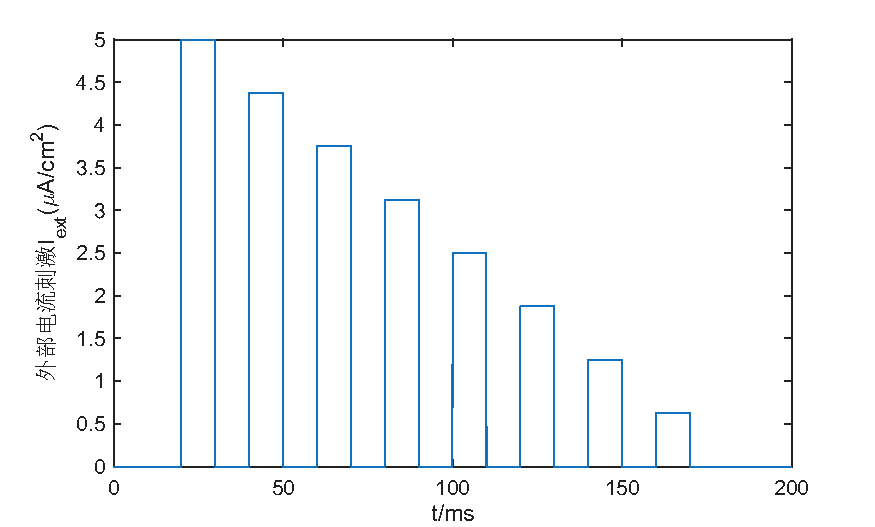
\includegraphics[width=\maxwidth{56.196688409433015em}]{figure_6.pdf}
\end{center}
\begin{matlaboutput}
下图是膜电压与时间的关系: 
\end{matlaboutput}
\begin{center}
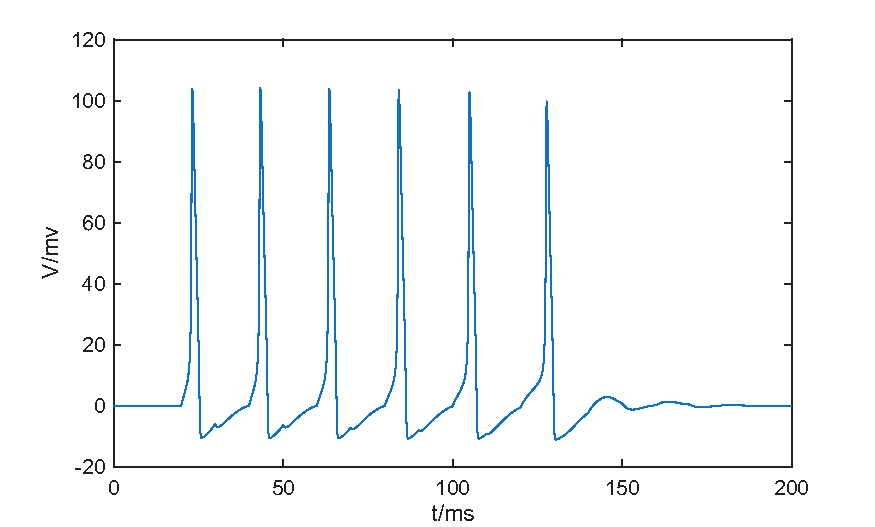
\includegraphics[width=\maxwidth{56.196688409433015em}]{figure_7.pdf}
\end{center}


\vspace{1em}


\vspace{1em}
\label{TMP_008e}
\matlabheadingtwo{直流刺激-使用文献中的参数和方程}

\begin{par}
\begin{flushleft}
《Energy and information in Hodgkin-Huxley neurons》A. Moujahid, A. d’Anjou, and F. J. Torrealdea
\end{flushleft}
\end{par}

\label{TMP_6c4e}
\begin{par}
\begin{flushleft}
中给出的参数是
\end{flushleft}
\end{par}

\begin{par}
\begin{flushleft}
电容:$C=1\mu {\textrm{F/cm}}^2$
\end{flushleft}
\end{par}

\begin{matlabcode}
clc;clear
C=1;
\end{matlabcode}

\begin{par}
\begin{flushleft}
各离子的能斯特电位和对应的电导:
\end{flushleft}
\end{par}

\begin{par}
$$\begin{array}{lrr}
\hline
x & E_x \;\textrm{[mV]} & g_x {\;\textrm{[mS}\;\textrm{/}\;\textrm{cm}}^2 \textrm{]}\\
\hline
\textrm{Na} & 115 & 120\\
\textrm{K} & -12 & 36\\
\textrm{L} & 10.6 & 0.3\\
\hline
\end{array}$$
\end{par}

\begin{matlabcode}
E.Na=115;E.K=-12;E.L=10.6;
g.Na=120;g.K=36;g.L=0.3;
\end{matlabcode}

\begin{par}
\begin{flushleft}
对应的 alpha和beta函数:
\end{flushleft}
\end{par}

\begin{par}
$$\begin{array}{lcc}
\hline
x & \alpha_x (u/\;\textrm{mV}){\;\textrm{[ms}}^{-1} \textrm{]} & \beta_x (u/\cdot \;\textrm{mV}){\;\textrm{[ms}}^{-1} \textrm{]}\\
\hline
n & (0.1-0.01u)/[\exp (1-0.1u)-1] & 0.125\exp (-u/80)\\
m & (2.5-0.1u)/[\exp (2.5-0.1u)-1] & 4\exp (-u/18)\\
h & 0.07\exp (-u/20) & 1/[\exp (3-0.1u)+1]\\
\hline
\end{array}$$
\end{par}

\begin{matlabcode}
Alpha.n=@(u) (0.1 - 0.01.*u) ./ (exp(1 - 0.1.*u) - 1);
Alpha.m=@(u) (2.5 - 0.1.*u) ./ (exp(2.5 - 0.1.*u) - 1);
Alpha.h=@(u) 0.07 .* exp(-u./20);
Beta.n=@(u) 0.125 .* exp(-u./80);
Beta.m=@(u) 4 .* exp(-u./18);
Beta.h=@(u) 1 ./ (exp(3 - 0.1.*u) + 1);
A=15;%刺激电流强度

fs= 4000;%采样频率
T=200;%总时长(ms)
I_ext = @(u) 0+(20<=u & u<= 150).*A;%脉冲刺激向量
[V,m,h,n]=Task1I2V(C,E,g,Alpha,Beta, ...
    'fs',fs, ...
    'T',T, ...
    'A',A, ...
    'I_ext',I_ext);
\end{matlabcode}
\begin{matlaboutput}
此时使用的参数为:
 C: 1.0000 
g的结构体:
    Na: 120
     K: 36
     L: 0.300000000000000

E的结构体:
    Na: 115
     K: -12
     L: 10.600000000000000

Alpha函数的结构体:
    n: @(u)(0.1-0.01.*u)./(exp(1-0.1.*u)-1)
    m: @(u)(2.5-0.1.*u)./(exp(2.5-0.1.*u)-1)
    h: @(u)0.07.*exp(-u./20)

Beta函数的结构体:
    n: @(u)0.125.*exp(-u./80)
    m: @(u)4.*exp(-u./18)
    h: @(u)1./(exp(3-0.1.*u)+1)

外部刺激电流:
    @(u)0+(20<=u&u<=150).*A


下图是外部电流刺激的时域图
\end{matlaboutput}
\begin{center}
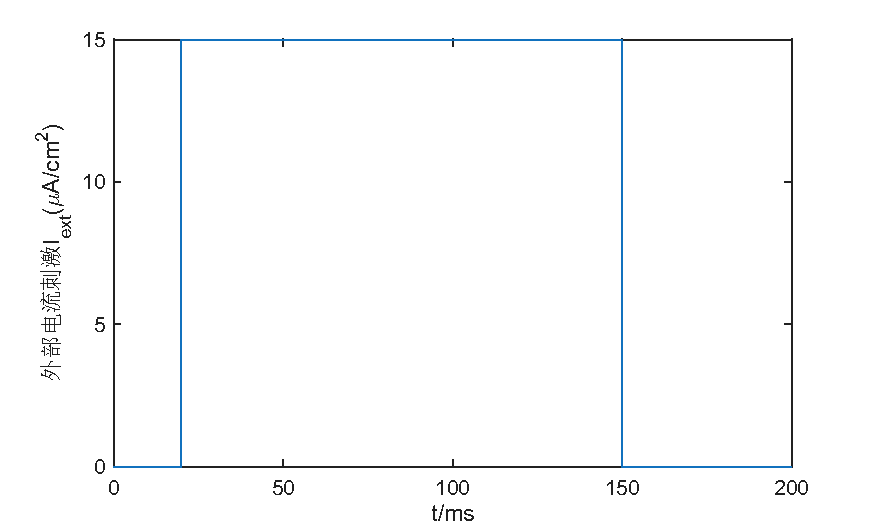
\includegraphics[width=\maxwidth{56.196688409433015em}]{figure_8.pdf}
\end{center}
\begin{matlaboutput}
下图是膜电压与时间的关系: 
\end{matlaboutput}
\begin{center}
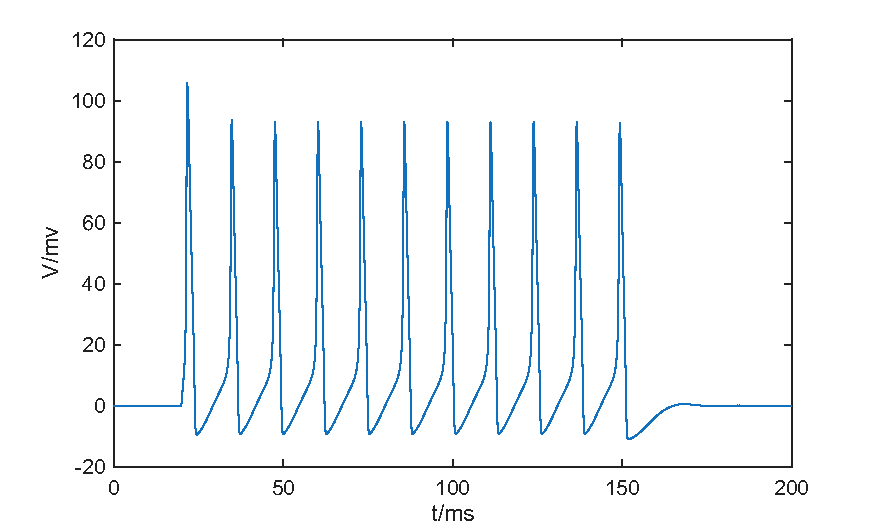
\includegraphics[width=\maxwidth{56.196688409433015em}]{figure_9.pdf}
\end{center}



\vspace{1em}
\label{TMP_3a43}
\matlabheading{任务 2:计算直流刺激强度和神经元发放频率之间的关系}


\vspace{1em}

\vspace{1em}
\begin{par}
\begin{flushleft}
  试计算直流刺激强度和神经元发放频率之间的关系   (提示: 神经元发放时间的确定)
\end{flushleft}
\end{par}


\vspace{1em}
\begin{par}
\begin{flushleft}
《Energy and information in Hodgkin-Huxley neurons》A. Moujahid, A. d’Anjou, and F. J. Torrealdea
\end{flushleft}
\end{par}

\label{TMP_6c4e}
\begin{par}
\begin{flushleft}
中给出的参数是
\end{flushleft}
\end{par}

\begin{par}
\begin{flushleft}
电容:$C=1\mu {\textrm{F/cm}}^2$
\end{flushleft}
\end{par}

\begin{matlabcode}
clc;clear
C=1;
\end{matlabcode}

\begin{par}
\begin{flushleft}
各离子的能斯特电位和对应的电导:
\end{flushleft}
\end{par}

\begin{par}
$$\begin{array}{lrr}
\hline
x & E_x \;\textrm{[mV]} & g_x {\;\textrm{[mS}\;\textrm{/}\;\textrm{cm}}^2 \textrm{]}\\
\hline
\textrm{Na} & 115 & 120\\
\textrm{K} & -12 & 36\\
\textrm{L} & 10.6 & 0.3\\
\hline
\end{array}$$
\end{par}

\begin{matlabcode}
E.Na=115;E.K=-12;E.L=10.6;
g.Na=120;g.K=36;g.L=0.3;
\end{matlabcode}

\begin{par}
\begin{flushleft}
对应的 alpha和beta函数:
\end{flushleft}
\end{par}

\begin{par}
$$\begin{array}{lcc}
\hline
x & \alpha_x (u/\;\textrm{mV}){\;\textrm{[ms}}^{-1} \textrm{]} & \beta_x (u/\cdot \;\textrm{mV}){\;\textrm{[ms}}^{-1} \textrm{]}\\
\hline
n & (0.1-0.01u)/[\exp (1-0.1u)-1] & 0.125\exp (-u/80)\\
m & (2.5-0.1u)/[\exp (2.5-0.1u)-1] & 4\exp (-u/18)\\
h & 0.07\exp (-u/20) & 1/[\exp (3-0.1u)+1]\\
\hline
\end{array}$$
\end{par}

\begin{matlabcode}
Alpha.n=@(u) (0.1 - 0.01.*u) ./ (exp(1 - 0.1.*u) - 1);
Alpha.m=@(u) (2.5 - 0.1.*u) ./ (exp(2.5 - 0.1.*u) - 1);
Alpha.h=@(u) 0.07 .* exp(-u./20);
Beta.n=@(u) 0.125 .* exp(-u./80);
Beta.m=@(u) 4 .* exp(-u./18);
Beta.h=@(u) 1 ./ (exp(3 - 0.1.*u) + 1);


%%计算静息电位时的初值(在大规模运算时为了提高性能而这样设计)
    fV=@(V,m,h,n,t) 1/C*(-g.L*(V-E.L)-g.Na*m^3*h*(V-E.Na)-g.K*n^4*(V-E.K)+I_ext(t));
    fm=@(V,m) Alpha.m(V)*(1-m)-Beta.m(V)*m;
    fh=@(V,h) Alpha.h(V)*(1-h)-Beta.h(V)*h;
    fn=@(V,n) Alpha.n(V)*(1-n)-Beta.n(V)*n;
    % 为了求解微分方程,我们还必须获得初始值,在静息时,I_ext肯定是0,V,m,h,n的导数也是零
    % 由此可以解方程数值求得初始值,同时也是静息值
    % 使用线性方程解出静息时的电位,各离子浓度比,此时I_ext肯定是0,所以得重新命名一个函数fVT来解方程
    
    syms V0 m0 h0 n0
    fVT=@(V,m,h,n) 1/C*(-g.L*(V-E.L)-g.Na*m^3*h*(V-E.Na)-g.K*n^4*(V-E.K)+0);
    eqt=[fVT(V0,m0,h0,n0),fm(V0,m0)==0,fh(V0,h0)==0,fn(V0,n0)==0];
    VPASol=vpasolve(eqt,[V0 m0 h0 n0]);


% fs= 6000;%采样频率
T=1000;%总时长(ms)
fs=13*T;%采样频率随时间增长而增加,这样可以有效避免解爆炸

DelA=0.5;
Amax=50;
Avec=0:DelA:Amax;
N_A=length(Avec);
fPkz=zeros(1,N_A);
i=1;

for A=0:DelA:Amax %刺激电流强度

I_ext = @(u) 0+(0.1*T<=u & u<= 0.9*T).*A;%脉冲刺激向量


[V,m,h,n]=Task2I2V_fast(C,E,g,Alpha,Beta,VPASol, ...
    'fs',fs, ...
    'T',T, ...
    'A',A, ...
    'I_ext',I_ext...
    );
Threold=max(V)*2/3;
% findpeaks(V.*(V>=Threold));
[pks,locs]=findpeaks(V.*(V>=Threold));
NPkz=length(pks);
fPkz(i)=NPkz/(0.8*T*1e-3);
% disp(fPkz)
i=i+1;
end
figure;
plot(Avec,fPkz)
xlabel('A (\muA/cm^2)'), ylabel('f/Hz')
\end{matlabcode}
\begin{center}
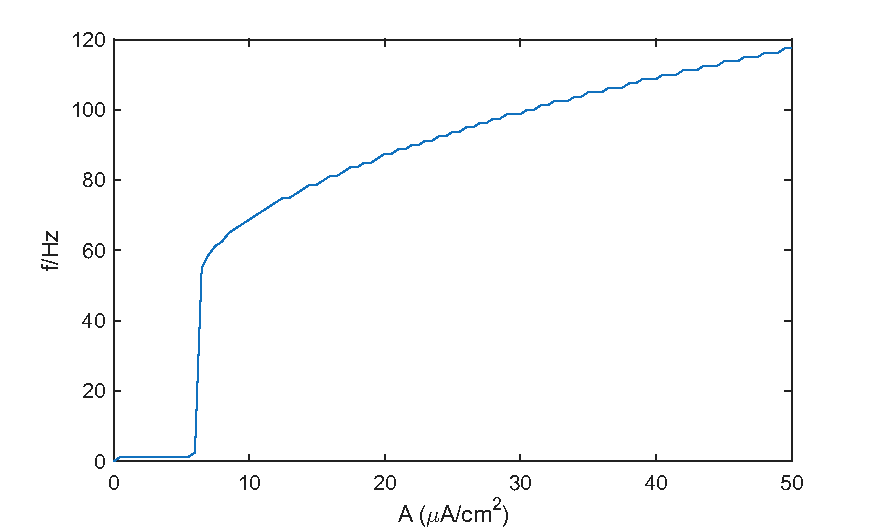
\includegraphics[width=\maxwidth{56.196688409433015em}]{figure_10.pdf}
\end{center}
\begin{matlabcode}

\end{matlabcode}



\vspace{1em}
\label{TMP_1357}
\matlabheading{任务 3:计算一个动作电势过程中的通过单位面积细胞膜的钠离子总数目}


\vspace{1em}

\vspace{1em}
\begin{par}
\begin{flushleft}
  试计算一个动作电势过程中的通过单位面积细胞膜的钠离子总数目  
\end{flushleft}
\end{par}


\vspace{1em}
\begin{par}
\begin{flushleft}
对一个动作电势过程中的钠电流进行积分, 得到通过钠离子通道的总电量, 除以元电荷电量  
\end{flushleft}
\end{par}


\vspace{1em}
\begin{par}
$$\left\lbrace \begin{array}{l}
C_m \frac{dV}{dt}=-g_L (V-E_L )-{\bar{g} }_{Na} m^3 h(V-E_{Na} )-{\bar{g} }_K n^4 (V-E_K )+I_{app} \\
\frac{dm}{dt}=\alpha_m (V)(1-m)-\beta_m (V)m\\
\frac{dh}{dt}=\alpha_h (V)(1-h)-\beta_h (V)h\\
\frac{dn}{dt}=\alpha_n (V)(1-n)-\beta_n (V)n
\end{array}\right.$$
\end{par}

\begin{par}
\begin{flushleft}
《Energy and information in Hodgkin-Huxley neurons》A. Moujahid, A. d’Anjou, and F. J. Torrealdea
\end{flushleft}
\end{par}

\label{TMP_6c4e}
\begin{par}
\begin{flushleft}
中给出的参数是
\end{flushleft}
\end{par}

\begin{par}
\begin{flushleft}
电容:$C=1\mu {\textrm{F/cm}}^2$
\end{flushleft}
\end{par}

\begin{matlabcode}
clc;clear
C=1;
\end{matlabcode}

\begin{par}
\begin{flushleft}
各离子的能斯特电位和对应的电导:
\end{flushleft}
\end{par}

\begin{par}
$$\begin{array}{lrr}
\hline
x & E_x \;\textrm{[mV]} & g_x {\;\textrm{[mS}\;\textrm{/}\;\textrm{cm}}^2 \textrm{]}\\
\hline
\textrm{Na} & 115 & 120\\
\textrm{K} & -12 & 36\\
\textrm{L} & 10.6 & 0.3\\
\hline
\end{array}$$
\end{par}

\begin{matlabcode}
E.Na=115;E.K=-12;E.L=10.6;
g.Na=120;g.K=36;g.L=0.3;
\end{matlabcode}

\begin{par}
\begin{flushleft}
对应的 alpha和beta函数:
\end{flushleft}
\end{par}

\begin{par}
$$\begin{array}{lcc}
\hline
x & \alpha_x (u/\;\textrm{mV}){\;\textrm{[ms}}^{-1} \textrm{]} & \beta_x (u/\cdot \;\textrm{mV}){\;\textrm{[ms}}^{-1} \textrm{]}\\
\hline
n & (0.1-0.01u)/[\exp (1-0.1u)-1] & 0.125\exp (-u/80)\\
m & (2.5-0.1u)/[\exp (2.5-0.1u)-1] & 4\exp (-u/18)\\
h & 0.07\exp (-u/20) & 1/[\exp (3-0.1u)+1]\\
\hline
\end{array}$$
\end{par}

\begin{matlabcode}
Alpha.n=@(u) (0.1 - 0.01.*u) ./ (exp(1 - 0.1.*u) - 1);
Alpha.m=@(u) (2.5 - 0.1.*u) ./ (exp(2.5 - 0.1.*u) - 1);
Alpha.h=@(u) 0.07 .* exp(-u./20);
Beta.n=@(u) 0.125 .* exp(-u./80);
Beta.m=@(u) 4 .* exp(-u./18);
Beta.h=@(u) 1 ./ (exp(3 - 0.1.*u) + 1);



fs= 4000;%采样频率
T=11;%总时长(ms)
A=15;%刺激电流强度
t=0:T/fs:T;%时间序列向量
Del=t(2)-t(1);%时间间隔
N=length(t);%时间离散化数量

I_ext = @(u) 0+(1<=u & u<= 10).*A;%脉冲刺激向量
[V,m,h,n]=Task3I2V(C,E,g,Alpha,Beta, ...
    'fs',fs, ...
    'T',T, ...
    'A',A, ...
    'I_ext',I_ext);
\end{matlabcode}
\begin{matlaboutput}
此时使用的参数为:
 C: 1.0000 
g的结构体:
    Na: 120
     K: 36
     L: 0.300000000000000

E的结构体:
    Na: 115
     K: -12
     L: 10.600000000000000

Alpha函数的结构体:
    n: @(u)(0.1-0.01.*u)./(exp(1-0.1.*u)-1)
    m: @(u)(2.5-0.1.*u)./(exp(2.5-0.1.*u)-1)
    h: @(u)0.07.*exp(-u./20)

Beta函数的结构体:
    n: @(u)0.125.*exp(-u./80)
    m: @(u)4.*exp(-u./18)
    h: @(u)1./(exp(3-0.1.*u)+1)

外部刺激电流:
    @(u)0+(1<=u&u<=10).*A


下图是外部电流刺激的时域图
\end{matlaboutput}
\begin{center}
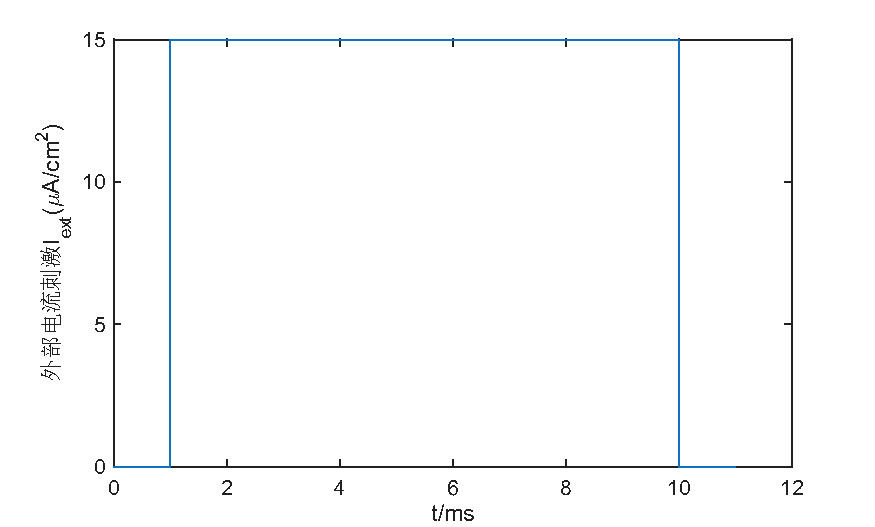
\includegraphics[width=\maxwidth{56.196688409433015em}]{figure_11.pdf}
\end{center}
\begin{matlaboutput}
下图是膜电压与时间的关系: 
\end{matlaboutput}
\begin{center}
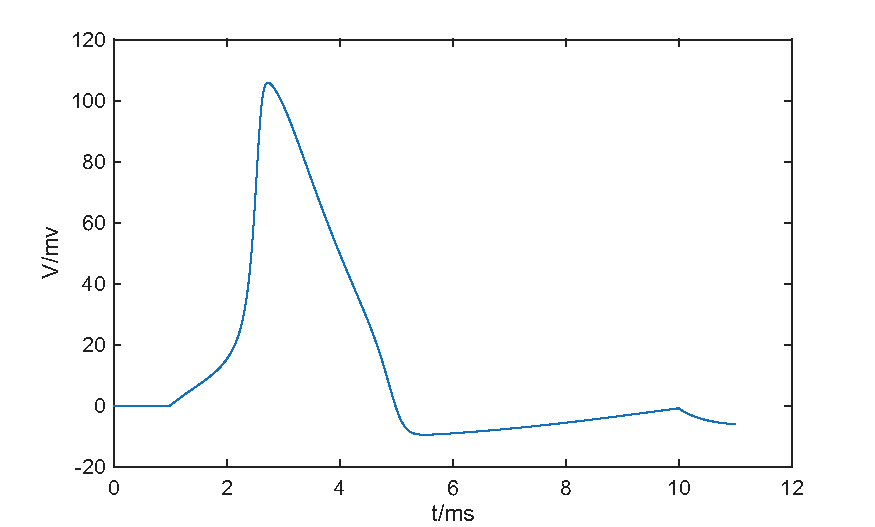
\includegraphics[width=\maxwidth{56.196688409433015em}]{figure_12.pdf}
\end{center}

\begin{par}
$$C_m \frac{dV}{dt}=-g_L (V-E_L )-{\bar{g} }_{Na} m^3 h(V-E_{Na} )-{\bar{g} }_K n^4 (V-E_K )+I_{app}$$
\end{par}

\begin{matlabcode}
I.K=-g.K.*n.^4.*(V-E.K);
I.L=-g.L.*(V-E.L);
I.Na=-g.Na.*m.^3.*h.*(V-E.Na);
figure;
plot(t,I.K,'b',t,I.L,'r',t,I.Na)
hold on
xlabel('t/ms')
ylabel('I(\muA/cm^2)')
legend('I_{K}','I_{L}','I_{Na}')
\end{matlabcode}
\begin{center}
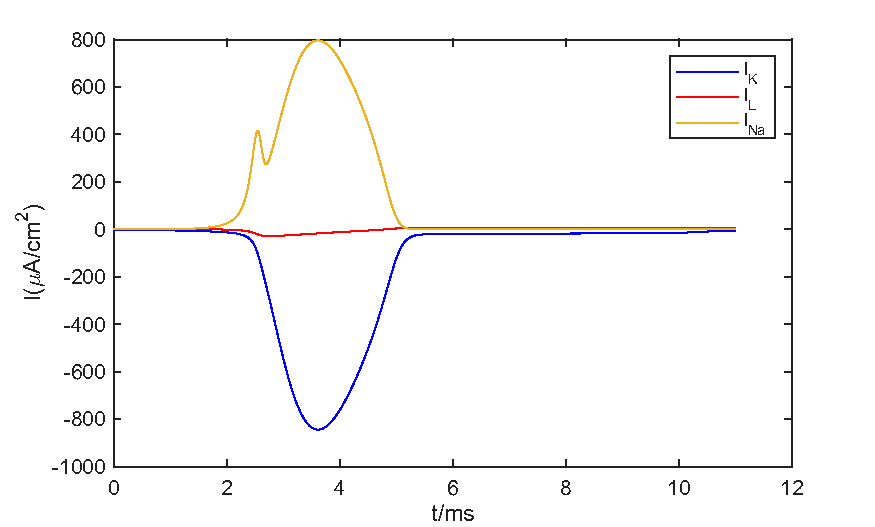
\includegraphics[width=\maxwidth{56.196688409433015em}]{figure_13.pdf}
\end{center}
\begin{matlabcode}

Qint.K=trapz(t,I.K);
Qint.L=trapz(t,I.L);
Qint.Na=trapz(t,I.Na);
fprintf('穿过膜的各离子电荷量(C):\n')
\end{matlabcode}
\begin{matlaboutput}
穿过膜的各离子电荷量(C):
\end{matlaboutput}
\begin{matlabcode}
disp(Qint)
\end{matlabcode}
\begin{matlaboutput}
     K: -1.540989404456195e+03
     L: -6.326641364649794
    Na: 1.406198873216253e+03
\end{matlaboutput}
\begin{matlabcode}
e=1.602176634e-19 %元电荷电量
\end{matlabcode}
\begin{matlaboutput}
e = 
     1.602176634000000e-19

\end{matlaboutput}
\begin{matlabcode}
Nint.K=Qint.K/e;
Nint.L=Qint.L/e;
Nint.Na=Qint.Na/e;
fprintf('穿过膜的各离子个数:\n')
\end{matlabcode}
\begin{matlaboutput}
穿过膜的各离子个数:
\end{matlaboutput}
\begin{matlabcode}
disp(Nint)
\end{matlabcode}
\begin{matlaboutput}
     K: -9.618099351561225e+21
     L: -3.948778948832052e+19
    Na: 8.776803027675741e+21
\end{matlaboutput}



\vspace{1em}
\label{TMP_3ac9}
\matlabheading{扩展:}

\begin{par}
\begin{flushleft}
如果 V 是膜电位,电路中在给定时刻累积的总电能为
\end{flushleft}
\end{par}

\begin{par}
$$H(t)=\frac{1}{2}CV^2 +H_{Na} +H_K +H_l ,~~(3)$$
\end{par}

\begin{par}
\begin{flushleft}
其中求和的第一项代表电容器中累积的电能,另外三项分别是电池中的能量。电池中累积的电化学能是未知的。在该模型中,它可能是无限的,因为我们没有考虑电池的耗尽。在真实的神经元中,营养物质的摄入防止了离子泵的耗尽。然而,已知电池向电路提供的电能速率是流过电池的电流乘以其电动势。因此,上述能量对时间的全导数将是
\end{flushleft}
\end{par}

\begin{par}
$$\dot{H} (t)=CV\dot{V} +i_{Na} E_{Na} +i_K E_K +i_l E_l .~~(4)$$
\end{par}

\begin{par}
\begin{flushleft}
设 $I$ 代表以某种方式注入膜的总外部电流。根据方程 (1) 中的第一个方程,我们有
\end{flushleft}
\end{par}

\begin{par}
$$C\dot{V} =I-i_{Na} -i_K -i_l ,$$
\end{par}

\begin{par}
\begin{flushleft}
将其代入方程 (4) 可得
\end{flushleft}
\end{par}

\begin{par}
$$\dot{H} =VI-i_{Na} (V-E_{Na} )-i_K (V-E_K )-i_l (V-E_l ).$$
\end{par}

\begin{par}
\begin{flushleft}
如果我们将方程 (2) 代入离子电流,我们得到电路中的能量速率为
\end{flushleft}
\end{par}

\begin{par}
$$\dot{H} =VI-g_{Na} m^3 h(V-E_{Na} )^2 -g_K n^4 (V-E_K )^2$$
\end{par}

\begin{par}
$$-g_l (V-E_l )^2 ,~~(5)$$
\end{par}

\begin{par}
\begin{flushleft}
这提供了神经元中电化学能量关于其状态变量的全导数。 右手边求和中的第一项表示通过到达神经元的不同连接 给予神经元的电功率,而求和中的其他三项表示离子通道每秒消耗的能量。由于发放率取决于总电流 I, 霍奇金赫胥黎神经元的平均代谢消耗作为发放率的函数可以通过简单评估式(5) 在不同外部电流值下 I。以下两节介绍了这些计算的结果。
\end{flushleft}
\end{par}


\vspace{1em}

\vspace{1em}
\begin{par}
\begin{flushleft}
PHYSICAL REVIEW E 83, 031912 (2011)
\end{flushleft}
\end{par}

\begin{par}
\begin{flushleft}
  Hodgkin-Huxley 神经元中的能量与信息  
\end{flushleft}
\end{par}

\begin{par}
\begin{flushleft}
A. Moujahid, A. d'Anjou, and F. J. Torrealdea
\end{flushleft}
\end{par}

\begin{par}
\begin{flushleft}
 西班牙 ES-20018 圣塞巴斯蒂安,巴斯克大学计算机科学系 
\end{flushleft}
\end{par}

\begin{par}
\begin{flushleft}
F. Torrealdea
\end{flushleft}
\end{par}

\begin{par}
\begin{flushleft}
 英国伦敦 WC1N 3BG,伦敦大学学院神经学研究所 
\end{flushleft}
\end{par}

\begin{par}
\begin{flushleft}
(2010 年 8 月 9 日收到;2011 年 1 月 21 日收到修订稿;2011 年 3 月 21 日发表)
\end{flushleft}
\end{par}

\begin{par}
\begin{flushleft}
---
\end{flushleft}
\end{par}


\vspace{1em}
\begin{par}
\begin{flushleft}
  对“Hodgkin-Huxley 神经元中的能量与信息”的评论  
\end{flushleft}
\end{par}

\begin{par}
\begin{flushleft}
Hideo Hasegawa 
\end{flushleft}
\end{par}

\begin{par}
\begin{flushleft}
 日本东京 184-8501 小金井市,东京学艺大学物理系 
\end{flushleft}
\end{par}

\begin{par}
\begin{flushleft}
(日期:2011 年 6 月 30 日)
\end{flushleft}
\end{par}

\begin{par}
\begin{flushleft}
  摘要  
\end{flushleft}
\end{par}

\begin{par}
\begin{flushleft}
在最近的一篇论文 [A. Moujahid, A. d'Anjou, F. J. Torrealdea and F. Torrealdea, Phys. Rev. E 83, 031912 (2011)] 中,作者们使用 Hodgkin-Huxley (HH) 模型(霍奇金-赫胥黎模型)计算了神经元放电时消耗的能量。HH 模型采用的能量消耗率得出了负的能量消耗,这意味着能量从 HH 神经元转移到了源,这在物理上是奇怪的,尽管他们将其解释为生化能量成本。我提出了功耗的另一种表达式,该表达式导致 HH 神经元消耗正能量,并提出了一些模型计算结果,与他们论文中的结果进行了比较。
\end{flushleft}
\end{par}

\begin{par}
\begin{flushleft}
PACS 分类号: 87.19.1l, 87.19.lg, 87.19.ly, 87.18.Sn
\end{flushleft}
\end{par}

\end{document}
